\documentclass{../notes}

\title{商务智能 HW02}

\begin{document}
    \maketitle

    \paragraph*{1} 参见PDF附件

    \paragraph*{2} MLP的结构图如图\ref{fig:network-structure}所示

    \begin{figure}[ht]
        \centering
        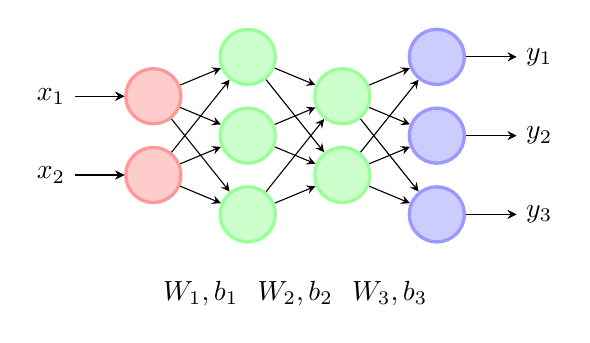
\begin{tikzpicture}
            [
                StartNode/.style={circle, draw=red!40, fill=red!20, very thick, minimum size = 7mm},
                HiddenNode/.style={circle, draw=green!40, fill=green!20, very thick, minimum size = 7mm},
                EndNode/.style={circle, draw=blue!40, fill=blue!20, very thick, minimum size = 7mm},
                Connection/.style={-stealth}
            ]
            \foreach \x in {1,2} {
                \node (A_\x) at (-1.3, -\x){$x_{\x}$};
                \node[StartNode] (a_\x) at (0, -\x){};
            }
            \foreach \x in {1,2,3}
                \node[HiddenNode] (b_\x) at (1.2, 0.5-\x){};
            \foreach \x in {1,2}
                \node[HiddenNode] (c_\x) at (2.4, -\x){};
            \foreach \x in {1,2,3} {
                \node[EndNode] (d_\x) at (3.6, 0.5-\x){};
                \node (B_\x) at (4.9, 0.5-\x){$y_{\x}$};
            }

            \foreach \x in {1,2,3} {
                \node (label_\x) at (-0.6 + 1.2 * \x, -3.5){$\bs W_\x, \bs b_\x$};
            }

            \foreach \x in {1,2,3} {
                \foreach \y in {1, 2} {
                    \draw[Connection] (A_\y) -> (a_\y);
                    \draw[Connection] (a_\y) -> (b_\x);
                    \draw[Connection] (b_\x) -> (c_\y);
                    \draw[Connection] (c_\y) -> (d_\x);
                    \draw[Connection] (d_\x) -> (B_\x);
                }
            }
        \end{tikzpicture}
        \caption{MLP网络结构}
        \label{fig:network-structure}
    \end{figure}

    设输入为$\bs X_0 = \begin{bmatrix} x_1 & x_2 \end{bmatrix}^\top $、输出为$\bs Y = \begin{bmatrix} y_1 & y_2 & y_3 \end{bmatrix}^\top$。Sigmoid函数为

    \begin{equation}
        f(\bs X) = \begin{bmatrix} \frac{1}{1 + e^{-x_1}} & \dots & \frac{1}{1 + e^{-x_n}} \end{bmatrix} ^\top
    \end{equation}

    Softmax函数为

    \begin{equation}
        g(\bs X) = \frac{x_{ij}}{\sum_{j} x_{ij}}
    \end{equation}

    交叉熵按照如下方式计算:

    \begin{equation}
        l(\bs X, \bs y) = -\sum_{i=1}^m \log \frac{e^{X_{i, y_i}}}{\sum_{j=1}^{n} e^{X_{ij}}}
    \end{equation}

    正向计算过程如下所示:

    \begin{equation}
        \begin{aligned}
            \text{第一个隐藏层的输出} & \bs X_1 = f(\bs a_1) = f(\bs W_1\bs X_0 + \bs b_1) \\
            \text{第二个隐藏层的输出} & \bs X_2 = f(\bs a_2) = f(\bs W_2\bs X_1 + \bs b_2) \\
            \text{输出层的输出} & \hat {\bs Y} = g(\bs a_3) = g(\bs W_3\bs X_2 + \bs b_3) \\
            \text{输出的分类标签} & \bs T = \arg\max_{i} \bs Y \\
            \text{损失函数} & \bs L = l(\bs Y)
        \end{aligned}
    \end{equation}

    反向传播过程如下所示,首先,设$f'(\bs X) = \frac{\dd f}{\dd \bs X}, g'(\bs X) = \frac{\dd g}{\dd \bs X}, l'(\hat {\bs Y}; \bs Y) = \frac{\partial l}{\partial \hat{\bs Y}}$,令$\bs 1 = \begin{bmatrix} 1 & \dots & 1\end{bmatrix}^\top$。由于Sigmoid函数、Softmax函数及交叉熵损失函数均为逐元素的计算,因此在反向求导时同样需要采取逐元素的矩阵运算,此处使用$\odot$表示逐元素的矩阵乘法。

    \begin{equation}
        \begin{aligned}
            \text{输出层的梯度} & \begin{cases}
                \bs g_3 &= l'(\hat {\bs Y}; \bs Y) \odot g'(\bs a_3) \\
                \nabla \bs W_3 &= \bs X_2^\top \bs g_3 \\
                \nabla \bs b_3 &= \bs 1^\top \bs g_3 \\
            \end{cases} \\
            \text{第二个隐藏层的梯度} & \begin{cases}
                \bs g_2 &= \left(\bs g_3 \bs W_3^\top\right) \odot f'(\bs a_2) \\
                \nabla \bs W_2 &= \bs X_1^\top \bs g_2 \\
                \nabla \bs b_2 &= \bs 1^\top \bs g_2 \\
            \end{cases} \\
            \text{第一个隐藏层的梯度} & \begin{cases}
                \bs g_1 &= \left(\bs g_2 \bs W_2^\top\right) \odot f'(\bs a_2) \\
                \nabla \bs W_1 &= \bs X_0^\top \bs g_1 \\
                \nabla \bs b_1 &= \bs 1^\top \bs g_1 \\
            \end{cases}
        \end{aligned}
    \end{equation}

    计算得到梯度后,按照学习率对参数进行优化,设学习率为$r$,则经过一步学习后的参数为:

    \begin{equation}
        \begin{aligned}
            \bs W_i' &= \bs W_i - r\nabla \bs W_i \\
            \bs b_i' &= \bs b_i - r\nabla \bs b_i \\
        \end{aligned}
    \end{equation}
\end{document}